\documentclass{if-beamer}

\usepackage[normalem]{ulem}

% --------------------------------------------------- %
%                  Presentation info	              %
% --------------------------------------------------- %
\title[Szybki wstęp do OpenMP]{Szybki wstęp do OpenMP}
\subtitle{czyli jak wycisnąć więcej z CPU i optymalizować równoległe obliczenia}
\author{Jan Iwaszkiewicz}
\institute[MFI]{
  Wydział Matematyki, Fizyki i Informatyki\\
  Uniwersytet Gdański
}
\date{30 kwietnia 2019}
% \logo{
% 
\includegraphics[scale=0.03]{flash_edit.png} % ZMIENIĆ
% }
\subject{OpenMP optymalizacja} % metadata

\graphicspath{{graphics/}}
% --------------------------------------------------- %
%                    Title + Schedule                 %
% --------------------------------------------------- %

\begin{document}

\usebackgroundtemplate{%
  
\includegraphics[scale=0.42]{flash_edit.png}} 
\begin{frame}
  \titlepage
\end{frame}

\usebackgroundtemplate{} 
\begin{frame}{Plan prezentacji}
  \tableofcontents
\end{frame}

% --------------------------------------------------- %
%                      Presentation                   %
% --------------------------------------------------- %
\section{Wstęp - czym jest OpenMP?}
\begin{frame}{Wstęp - czym jest OpenMP?}

\begin{columns}

\begin{column}{0.6\textwidth}
\textbf{\exemple{OpenMP}} to interfejs umożliwiający tworzenie programów dla systemów wieloprocesorowych. \emph{Dostępny dla języków C, C++ oraz Fortran.} Dostosowany do wielu architektur, w tym też Unixowych. Składa się ze zbioru dyrektyw kompilatora, bibliotek i zmiennych środowiskowych.
\end{column}

\begin{column}{0.4\textwidth}

\begin{figure}
\centering

\includegraphics[scale=0.1]{openmp.png}
\caption{Logo OpenMP, skrót HPC oznacza High-performance Computing.}
\end{figure}

\end{column}

\end{columns}
\end{frame}

\section{Teoria}

\subsection{Czy warto zrównoleglić obliczenia?}

\usebackgroundtemplate{%
  
\includegraphics[scale=0.40]{yoda_edit.png}} 
\begin{frame}{PARDOn't}
\boxblue{
\centering
{\huge O wszystkim zapomnij czego nauczyłeś się! \linebreak \linebreak \linebreak \linebreak } {\footnotesize Prawie wszystkim.}}
\end{frame}

\usebackgroundtemplate{} 
\begin{frame}{PARDOn't}

\begin{block}{Za}
\begin{itemize}
  \item Problem jest łatwy do zrównoleglenia
  \item Problem jest wystarczająco "duży"
  \item Dostęp do wyspecjalizowanego hardware (np. karty graficzne)
\end{itemize}
\end{block}

\begin{alertblock}{Przeciw}
\begin{itemize}
  \item "Skomplikowany" problem (np. brak możliwości ominięcia instrukcji warunkowych)
  \item Problem jest "mały" lub zbyt "prosty"
  \item Długi czas designu i optymalizacji takiego rozwiązania
\end{itemize}
\end{alertblock}
\end{frame}

\subsection{Praktyczne podejście}

\begin{frame}{Ograniczenia sprzętowe}

\begin{figure}
\centering
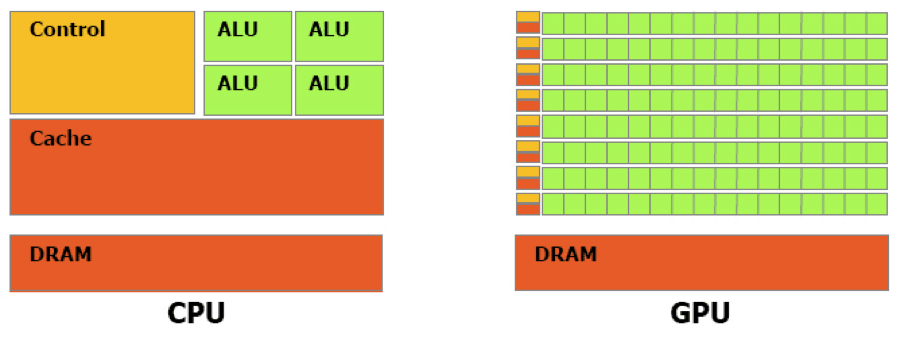
\includegraphics[scale=0.65]{cpuvsgpu.png}
\caption{Porównanie budowy CPU i GPU.}
\end{figure}

\end{frame}

\begin{frame}{"Z dedykacją..." - design algorytmów}

\emph{Cel algorytmu, rozmiar i typ danych wejściowych, docelowy hardware, a nawet koszt zasilania sprzętu może mieć wpływ na wybrane rozwiązania przy tworzeniu kodu.} Każdy nowy czynnik może drastycznie obniżyć jakość stworzonego programu.

\begin{block}{Gdzie szukać inspiracji?}
\begin{itemize}
  \item LAPACK - Linear Algebra PACKage
  \item Intel$^{®}$ Math Kernel Library for Deep Neural Networks (Intel$ ^{®}$ MKL-DNN)
  \item Eigen
\end{itemize}
  oraz wiele innych...
\end{block}

\end{frame}

\section{Pamięć}

\subsection{Ciągły dostęp do pamięci}

\begin{frame}{1 > 2 > 3 ... - zapis tablicy/wektora/tensora}

\begin{figure}
\centering
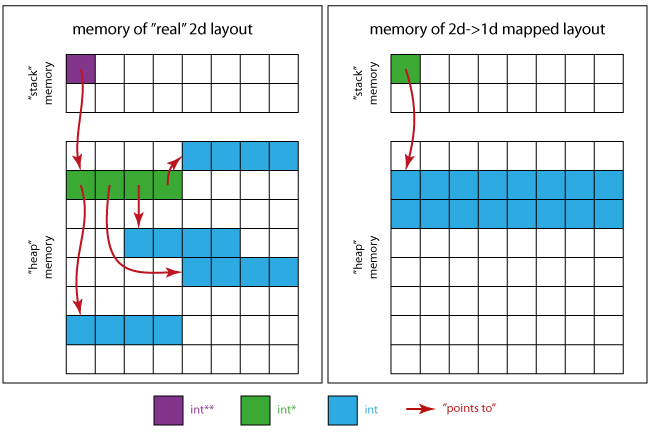
\includegraphics[scale=0.35]{1d2d.png}
\caption{Zapis tablicy dwu-wymiarowej i jedno-wymiarowej w pamięci.}
\end{figure}
  
\end{frame} 

\begin{frame}{1 > 2 > 3 ... - jak iterować?}

\begin{figure}
\centering
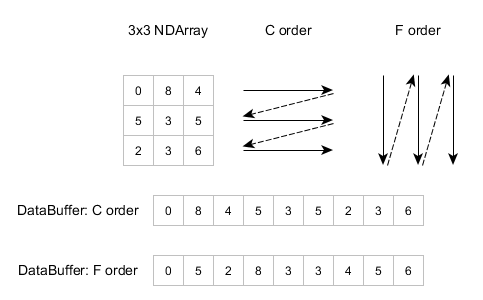
\includegraphics[scale=0.45]{rowcolwise.png}
\caption{Zapisywanie pamięci rzędami oraz kolumnami w różnych językach programowania.}
\end{figure}
  
\end{frame}

\subsection{Cache, cache i jeszcze raz cache}

\begin{frame}{Droga od RAM do procesora}

\begin{figure}
\centering
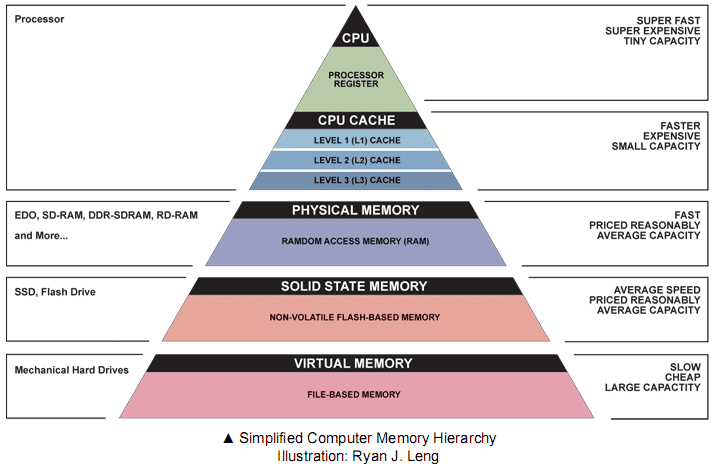
\includegraphics[scale=0.4]{memoverview.png}
\caption{Hierarchia pamięci.}
\end{figure}

\end{frame}

\begin{frame}{Droga od RAM do procesora}

\begin{figure}
\centering
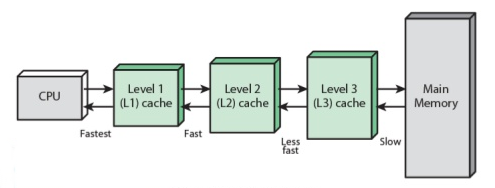
\includegraphics[scale=0.55]{memclose.png}
\caption{Droga jaką przebywają dane.}
\end{figure}

\end{frame}

\begin{frame}{We wnętrzu CPU}

\begin{figure}
\centering
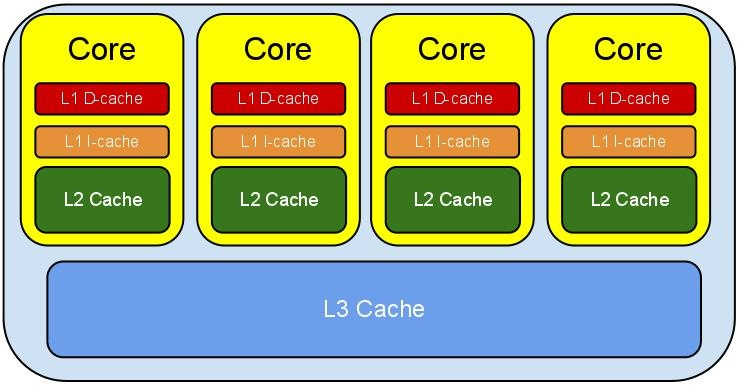
\includegraphics[scale=0.4]{memcpu.png}
\caption{Uproszczony szkic podziału pamięci CPU.}
\end{figure}

\end{frame}

\begin{frame}{Cache line}

\textbf{\exemple{Cache line}} to najnajmniejszy blok danych transferowany i przechowywany w pamięci podręcznej. Żeby dowiedzieć się jaki rozmiar linii jest przyjęty w danym procesorze, pod Linuxem, wystarczy wywołać komendę:
  
\code{ \textbf{{\footnotesize cat /sys/devices/system/cpu/cpu0/cache/index0/coherency\_line\_size}}}

Najbardziej typowy rozmiar to \emph{64B}, jednak zdarzają się też rozmiary od 32B do 256B.

\end{frame} 

\begin{frame}{False sharing}

\textbf{\exemple{False sharing}} niepożądane zjawisko podczas odczytu i zapisu danych przez różne wątki. \emph{Wątki pracujące na tym samym cache line mogą doprowadzić do stalling'u} (zastoju w transferze danych) poprzez ciągłe żądania aktualizacji danych.

\begin{figure}
\centering
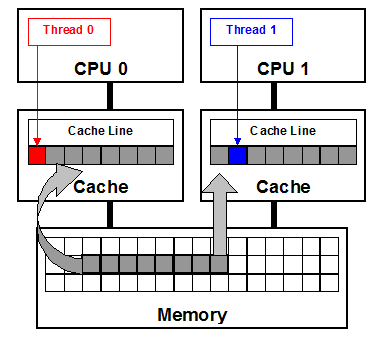
\includegraphics[scale=0.4]{false-sharing.png}
\caption{Przykład momentu, w którym zachodzi false sharing.}
\end{figure}
  
\end{frame} 

\begin{frame}{\sout{Garbage collector}}

Dlaczego większość wydajnych aplikacji wielowątkowych oraz matematycznych nie korzysta z "nowych" języków programowania? Jednym z minusów jest garbage collector.

\begin{alertblock}{Problemy}
\begin{itemize}
  \item Możliwość zatrzymania całego programu na czas działania - brak utylizacji pożądanej ciągłej wielwątkowości
  \item Koszt pracy garbage collector'a samego w sobie (szczególnie dawniej) - proces zajmuje cenny dla HPC czas 
  \item Zdarzają się zmiany w adresowaniu - przemieszczanie danych
\end{itemize}
\end{alertblock}
  
\end{frame} 

\section{Synchronizacja i Pseudo-CRCW}

\subsection{Synchronizacja wątków}

\begin{frame}{Bariery}

\code{\#pragma omp barrier}

\begin{figure}
\centering
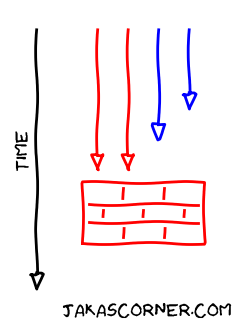
\includegraphics[scale=0.4]{bariera.png}
\caption{Szkic działania baiery, czerwone wątki natrafiły już na blokadę, niebieskie dalej pracują.}
\end{figure}

\end{frame}

\subsection{Pseudo-CRCW}

\begin{frame}{Odczyt danych - współdzielona pamięć}

\code{\#pragma omp ... shared(a, b, c)}
\centering
Podczas odczytu nie wystąpią żadne konfilkty.

\end{frame}

\begin{frame}{Zapis danych - operacje atomiczne}
\code{\#pragma omp atomic}
\code{\#pragma omp critical}
\centering
Podczas zapisu nie wystąpią żadne konfilkty. Jednak takie rozwiązanie prowadzi to do \emph{serializacji} zapisów i znaczącego spowolnienia działania programu.

\end{frame}

\section{Przykłady}
\subsection{Przykłady - prezentacja programów}
\begin{frame}
\frametitle{Przykłady - programy}

\begin{block}{Przykładowe operacje}
\begin{itemize}
  \item Dodawanie dwóch wektorów - $O(n)$
  \item Iloczyn skalarny dwóch wektorów - $O(n)$ 
  \item Mnożenie dwóch kwadratowych macierzy - $O(n^{3})$
\end{itemize}
\end{block}

\centering
Spójrzmy jak działają przygotowane przykłady i omówmy ich działanie.

\end{frame}

\subsection{Przykłady - optymalizacje kompilatora}
\begin{frame}[fragile]

\frametitle{Flagi kompilatora}

\centering
Spróbujmy zoptymalizować kod przy pomocy kompilatora, użyjmy do tego flag:

\code{-O3 -funroll-loops}
\blfootnote{\href{https://gcc.gnu.org/onlinedocs/gcc/Optimize-Options.html?fbclid=IwAR2YXJ7tPN0nU1r3xm\_p36LPmPCy4P3LiJ6j4bZQFfCeun6RhHIVvZ2FfQY}{Link do opisu flag dla kompilatora GCC}}
\end{frame}

\section{Podsumowanie}
\begin{frame}{Podsumowanie}

\centering
\begin{Large}
Dziękuję za uwagę! \linebreak Zapraszam do dyskusji oraz pytań.
\end{Large}
\end{frame}

% \section{Bibliografia}

\end{document}
